\section{Nivel 2 --- Control regulatorio}
\begin{frame}{Nivel 2: objetivo}
  \begin{block}{Función del control regulatorio}
    Genera comandos de \textbf{torque} $T_{tm}^*$ a partir de referencias de \textbf{velocidad} $v_t^*$ provenientes del Nivel 1 (supervisor)
  \end{block}

  \begin{block}{Objetivos de control}
    \begin{itemize}
      \item Seguimiento preciso de referencias de velocidad
      \item Suavidad en la respuesta transitoria
      \item Atenuación de perturbaciones: balanceo de carga, variaciones de masa
      \item Operación en tiempo discretizado (muestreado)
    \end{itemize}
  \end{block}

  \vspace{0.2cm}
  \begin{alertblock}{Estrategia de control}
    \textbf{Lazo regulador PI} + \textbf{compensaciones} (anti-windup) para mejorar respuesta ante saturación y frenos
  \end{alertblock}
\end{frame}

\begin{frame}{Modelo del carro para control de velocidad}
  \begin{block}{Dinámica simplificada de traslación}
    Se desprecian dinámicas rotacionales internas del accionamiento y se agrupan perturbaciones externas:
    \[
    M_t\,\frac{dv_t(t)}{dt} + b_t\,v_t(t) = F_{\text{cmd}}(t) + F_{\text{pert}}(t)
    \]
  \end{block}

  \vspace{-0.2cm}
  \begin{block}{Términos de la ecuación}
    \begin{itemize}
      \item $F_{\text{cmd}}(t) = K_f \, T_{tm}(t)$ con $K_f = \frac{i_t}{r_{td}}$ (conversión torque → fuerza)
      \vspace{0.05cm}
      \item $F_{\text{pert}}(t) = 2F_{hw}(t)\sin(\theta_l(t)) + T_{tb}(t,\text{BRK}_t) K_f$ 
      \begin{itemize}
        \item Componente horizontal del cable (acoplamiento)
        \item Fricción del freno de operación
      \end{itemize}
    \end{itemize}
  \end{block}

  \begin{alertblock}{Aproximación para diseño}
    Se descuida la fricción viscosa $b_t$ frente a la inercia dominante:
    \[
    G_{vel,t}(s) \approx \frac{K_f}{M_t\,s}
    \]
  \end{alertblock}
\end{frame}

\begin{frame}{Función de transferencia completa}
  \begin{block}{Planta sin aproximación}
    \[
    G_{vel,t}(s) = \frac{V_t(s)}{T_{tm}(s)} = \frac{K_f}{M_t\,s + b_t}
    \]
    con polo mecánico $P_{\text{mec}} = -\frac{b_t}{M_t}$ (pequeño en magnitud)
  \end{block}

  \vspace{-0.1cm}
  \begin{block}{Transformada de Laplace}
    Aplicando a la ecuación del carro:
    \[
    M_t\,s\,V_t(s) + b_t\,V_t(s) = K_f\,T_{tm}(s) + F_{\text{pert}}(s)
    \]
    Despejando $V_t(s)$:
    \[
    V_t(s) = \frac{K_f}{M_t\,s + b_t} \, T_{tm}(s) + \frac{1}{M_t\,s + b_t} \, F_{\text{pert}}(s)
    \]
  \end{block}

  \begin{alertblock}{Justificación de la aproximación}
    Como $b_t \ll M_t \, \omega_n$, el polo en $-b_t/M_t$ está muy alejado del eje jw. Se desprecia para simplificar el diseño.
  \end{alertblock}
\end{frame}

\begin{frame}{Diseño del controlador PI: especificación}
  \begin{block}{Tipo de controlador}
    Proporcional-integral (PI):
    \[
    C_{\text{vel}}(s) = K_p + \frac{K_i}{s}
    \]
  \end{block}

  \vspace{-0.1cm}
  \begin{block}{Beneficios del PI}
    \begin{itemize}
      \item Error nulo ante escalones de referencia de velocidad
      \item Buen rechazo de perturbaciones constantes (gravedad, fricción estática)
      \item Estructura simple, fácil de sintonizar
    \end{itemize}
  \end{block}

  \vspace{0.1cm}
  \begin{block}{Función de transferencia a lazo cerrado}
    \[
    T(s) = \frac{C_{\text{vel}}(s) \, G_{vel,t}(s)}{1 + C_{\text{vel}}(s) \, G_{vel,t}(s)} = \frac{K_p K_f\,s + K_i K_f}{M_t\,s^2 + K_p K_f\,s + K_i K_f}
    \]
  \end{block}
\end{frame}

\begin{frame}{Asignación de polos: ecuación característica}
  \begin{block}{Polinomio característico deseado de 2do orden}
    \[
    s^2 + 2\zeta\omega_n\,s + \omega_n^2
    \]
    con amortiguamiento $\zeta$ y frecuencia natural $\omega_n$
  \end{block}

  \vspace{-0.1cm}
  \begin{block}{Ecuación característica del lazo cerrado}
    \[
    M_t\,s^2 + K_p K_f\,s + K_i K_f = 0
    \]
    Dividiendo por $M_t$:
    \[
    s^2 + \frac{K_p K_f}{M_t}\,s + \frac{K_i K_f}{M_t} = 0
    \]
  \end{block}

  \vspace{-0.1cm}
  \begin{block}{Comparación e igualación de coeficientes}
    \begin{align*}
      \frac{K_p K_f}{M_t} &= 2\zeta\omega_n \quad \Rightarrow \quad K_p = \frac{2\zeta\omega_n M_t}{K_f} \\[4pt]
      \frac{K_i K_f}{M_t} &= \omega_n^2 \quad \Rightarrow \quad K_i = \frac{\omega_n^2 M_t}{K_f}
    \end{align*}
  \end{block}
\end{frame}

\begin{frame}{Parámetros de sintonía}
  \begin{block}{Selección de $\omega_n$ y $\zeta$}
    \begin{itemize}
      \item $\omega_n = 0.8$ rad/s: ancho de banda elegido en función de
      \begin{itemize}
        \item Limitaciones de aceleración del carro
        \item Compensación de perturbaciones
        \item Margen entre $\omega_n$ y dinámicas de orden superior (moduladores, sensores)
      \end{itemize}
      \vspace{0.1cm}
      \item $\zeta = 1$ (amortiguamiento crítico): \textbf{sin sobrepaso}
      \begin{itemize}
        \item Respuesta rápida pero suave
        \item Evita oscilaciones en la velocidad
        \item Reduce estrés mecánico
      \end{itemize}
    \end{itemize}
  \end{block}

  \vspace{0.1cm}
  \begin{alertblock}{Ganancias finales}
    \[
    K_p = \frac{2 \cdot 1 \cdot 0.8 \cdot M_t}{K_f} = \frac{1.6 M_t}{K_f}
    \quad ; \quad
    K_i = \frac{0.8^2 \cdot M_t}{K_f} = \frac{0.64 M_t}{K_f}
    \]
  \end{alertblock}
\end{frame}

\begin{frame}{Implementación discreta: ecuación de diferencias}
  \begin{block}{Transformación continuo → discreto}
    El controlador se implementa en tiempo discreto con período de muestreo $T_s$ (Nivel 2):
  \end{block}

  \vspace{-0.15cm}
  \begin{block}{Comando de torque en tiempo discreto}
    \[
    T_{tm}^*(k) = K_p\,e_v(k) + K_i \sum_{j=1}^{k} \frac{T_s}{2}\left[e_v(j) + e_v(j-1)\right]
    \]
    donde el error de velocidad es:
    \[
    e_v(k) = v_t^* - v_t(k)
    \]
  \end{block}

  \vspace{-0.1cm}
  \begin{block}{Integración numérica}
    Se usa la \textbf{regla del trapecio} para integración de la acción integral, mejorando precisión respecto a Euler
  \end{block}

  \begin{alertblock}{Recuerdo}
    Esta señal $T_{tm}^*(k)$ es la entrada al \textbf{modulador de torque} (limitación + filtro 1er orden)
  \end{alertblock}
\end{frame}

\begin{frame}{Anti-windup: concepto}
  \begin{block}{Problema: integrador sin reset}
    La presencia del \textbf{freno de operación} $\text{BRK}_t$ crea una situación donde:
    \begin{itemize}
      \item Cuando el freno está cerrado ($\text{BRK}_t = 0$), el accionamiento no puede acelerar
      \item Pero el término integral sigue acumulando error: $\sum e_v(k) \to \infty$
      \item Al abrir el freno, la salida del integrador es muy grande
      \item Resultado: sobreesfuerzos y respuesta lenta/inestable
    \end{itemize}
  \end{block}

  \vspace{0.1cm}
  \begin{alertblock}{Solución: reset del integrador}
    Se usa la \textbf{señal del freno negada} ($\overline{\text{BRK}_t}$) como reset de tipo \textit{level} en el integrador:
    \begin{itemize}
      \item Cuando $\text{BRK}_t = 0$ (freno cerrado): integrador se mantiene en cero
      \item Cuando $\text{BRK}_t = 1$ (freno abierto): integrador acumula error normalmente
    \end{itemize}
  \end{alertblock}
\end{frame}

\begin{frame}{Diagrama de bloques: Controlador PI del carro}
  \centering
  \begin{itemize}
    \item Entrada: referencia $v_t^*$ y velocidad medida $v_t(k)$ del encoder
    \item Error: $e_v(k) = v_t^* - v_t(k)$
    \item Rama proporcional: $K_p \, e_v(k)$
    \item Rama integral: $K_i \, I(k)$ con reset cuando $\text{BRK}_t = 0$
    \item Salida: $T_{tm}^*(k)$ saturado en $[-T_{tm\max}, +T_{tm\max}]$
  \end{itemize}

  \vspace{0.3cm}
  \begin{block}{Simulink}
    Ver diagrama en \texttt{nivel\_2/lazo\_controlador\_carro.png}
  \end{block}
\end{frame}

% Bruno Seccion 5.2 Diseño del Controlador de Balanceo
% \defaultmode
\begin{frame}{Control de balanceo (Anti-Sway): estrategia}
  \begin{block}{Control desacoplado (no basado en el modelo completo)}
    Se aprovechan dos dinámicas con escalas de tiempo \textbf{muy separadas}:
    \begin{itemize}
      \item \textbf{Accionamiento del carro}: rápido (establecimiento $< 100$ ms).
      \item \textbf{Péndulo de la carga}: lento (periodo natural $2$--$12$ s, según $l_h$).
    \end{itemize}
  \end{block}

  \begin{block}{Hipótesis de desacople}
    Con el lazo de velocidad bien sintonizado, $v_t(t) \approx v_t^*(t)$: la dinámica del
    actuador se separa de la pendular.
  \end{block}

  \begin{alertblock}{Idea}
    El balanceo se amortigua \textbf{modulando la velocidad de referencia} del carro, no con un
    actuador extra.
  \end{alertblock}
\end{frame}

\begin{frame}{Deducción de la ley de control no lineal}
  \begin{block}{Péndulo excitado por la aceleración del carro}
    \[
    \ddot\theta_l = -\frac{g}{l_h}\sin\theta_l - \frac{\ddot x_t}{l_h}\cos\theta_l
    \]
  \end{block}

  \vspace{-0.15cm}
  \begin{block}{Ley antibalanceo proporcional al ángulo}
    $v_t^* = v_{t\,target} + v_{sway}$, \quad con $\;v_{sway} = K_{sway}\,\theta_l$ \quad
    $\Rightarrow\; \ddot x_t \approx \dot v_{t\,target} + K_{sway}\,\dot\theta_l$.
    \[
    \ddot\theta_l + \underbrace{\left(\tfrac{K_{sway}}{l_h}\cos\theta_l\right)}_{\text{amortiguamiento}}\dot\theta_l
    + \frac{g}{l_h}\sin\theta_l = -\frac{\dot v_{t\,target}}{l_h}\cos\theta_l
    \]
  \end{block}

  \begin{alertblock}{Resultado clave}
    La velocidad inyectada se vuelve un \textbf{amortiguamiento viscoso no lineal}. Como
    $\cos(\theta_l) > 0$, es estable a cualquier ángulo operativo \textbf{sin} aproximar
    $\sin\theta_l\approx\theta_l$.
  \end{alertblock}
\end{frame}

\begin{frame}{Sintonía por linealización local (gain scheduling)}
  \begin{block}{Dinámica local ($\theta_l \approx 0$)}
    \begin{columns}[c]
      \begin{column}{0.4\textwidth}
        \[
        \ddot\theta_l + \frac{K_{sway}}{l_h}\dot\theta_l + \frac{g}{l_h}\theta_l = 0
        \]
        Comparando con $s^2 + 2\zeta\omega_n s + \omega_n^2$, con $\omega_n=\sqrt{g/l_h}$:
        \[
        \boxed{\,K_{sway}(l_h) = 2\,\zeta \,\sqrt{g \, l_h(t)}\,}
        \]
        \textbf{Gain scheduling}: $K_{sway}$ se ajusta con la longitud del cable $l_h$.
      \end{column}
      \begin{column}{0.48\textwidth}
        % \raggedleft
        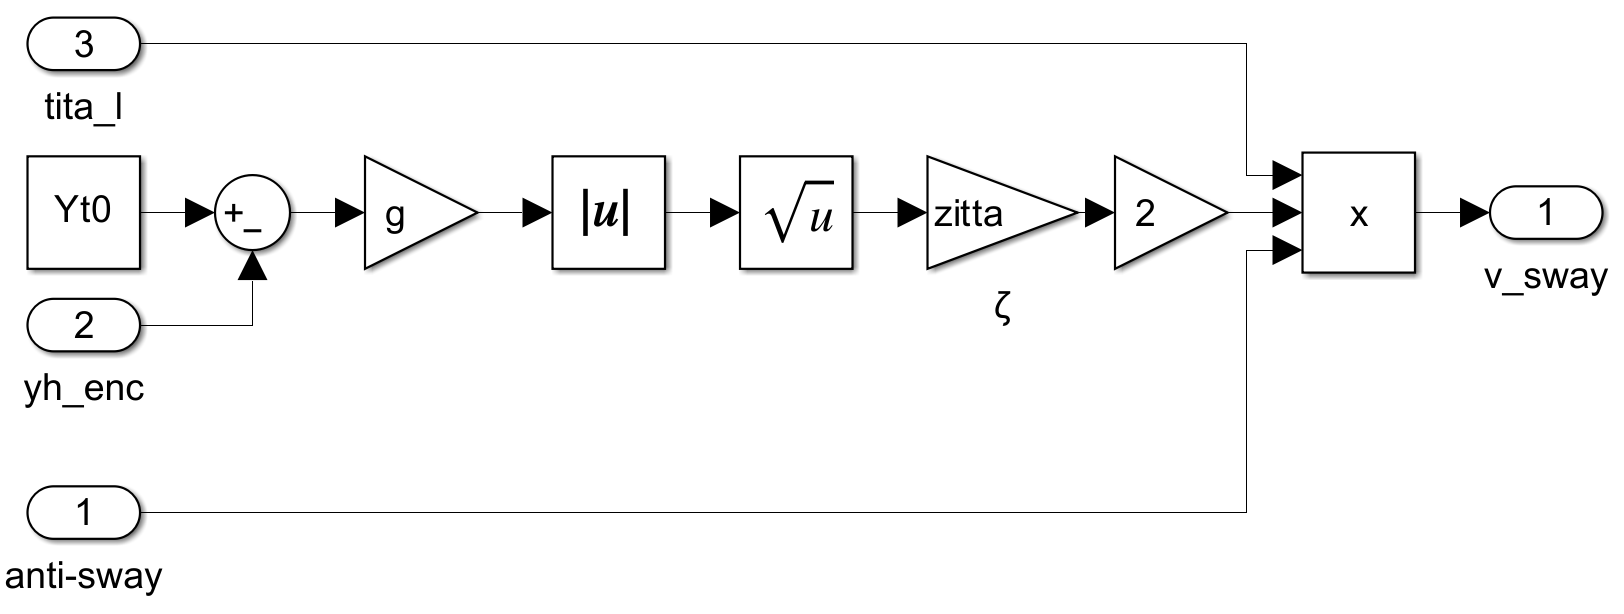
\includegraphics[width=0.8\linewidth]{nivel_2/control_balanceo.png}
      \end{column}
    \end{columns}
  \end{block}

  \begin{alertblock}{En la práctica}
    El amortiguamiento crítico ($\zeta=1$) sobrecorrige la posición; se usa $\zeta = 0.5$
    (subamortiguado) para mantener la carga cerca del objetivo.
  \end{alertblock}
\end{frame}

% \lautimode
\begin{frame}{Observador de estado del carro: motivación}
  \begin{block}{Problema de medición}
    \begin{itemize}
      \item Encoder mide solo \textbf{posición angular} $\theta_{tm}(t)$
      \item El controlador PI necesita \textbf{velocidad angular} $\omega_{tm}(t)$
      \item No se puede derivar la posición directamente (ruido, inestabilidad)
    \end{itemize}
  \end{block}

  \vspace{0.1cm}
  \begin{alertblock}{Solución}
    Implementar un \textbf{observador de estado} que estime $\tilde{\omega}_{tm}(t)$ a partir de la medición de $\theta_{tm}(t)$
  \end{alertblock}

  \vspace{0.2cm}
  \begin{block}{Complicación adicional}
    El observador convencional presenta \textbf{error en régimen permanente} ante perturbaciones constantes (balanceo de carga)
    \begin{itemize}
      \item Solución: agregar \textbf{acción integral} sobre el error de observación
    \end{itemize}
  \end{block}
\end{frame}

\begin{frame}{Modelo del carro en forma de estado}
  \begin{block}{Sistema simplificado (de la Ec. del accionamiento del carro)}
    \[
    \begin{cases}
      \dot{\theta}_{tm}(t) = \omega_{tm}(t) \\[6pt]
      \dot{\omega}_{tm}(t) = -\frac{b_{t,eq}}{J_{t,eq}}\omega_{tm}(t) + \frac{1}{J_{t,eq}}T_{tm}^*(t)
    \end{cases}
    \]
  \end{block}

  \vspace{-0.1cm}
  \begin{block}{Forma matricial: $\dot{\mathbf{x}} = A\mathbf{x} + B_c u$ ; $y = C\mathbf{x}$}
    \[
    \begin{bmatrix}
      \dot{\theta}_{tm}(t) \\
      \dot{\omega}_{tm}(t)
    \end{bmatrix}
    =
    \begin{bmatrix}
      0 & 1 \\
      0 & -\frac{b_{t,eq}}{J_{t,eq}}
    \end{bmatrix}
    \begin{bmatrix}
      \theta_{tm}(t) \\
      \omega_{tm}(t)
    \end{bmatrix}
    +
    \begin{bmatrix}
      0 \\
      \frac{1}{J_{t,eq}}
    \end{bmatrix}
    T_{tm}^*(t)
    \]
    \[
    y(t) = \begin{bmatrix} 1 & 0 \end{bmatrix}
    \begin{bmatrix}
      \theta_{tm}(t) \\
      \omega_{tm}(t)
    \end{bmatrix}
    = \theta_{tm}(t)
    \]
  \end{block}
\end{frame}

\begin{frame}{Problema: error del observador en régimen permanente}
  \begin{block}{Observador de Luenberger convencional}
    \[
    \dot{\hat{\mathbf{x}}} = (A - K_e C) \hat{\mathbf{x}} + B_c u + K_e y
    \]
    con matriz de ganancia $K_e = \begin{bmatrix} k_{\theta t} \\ k_{\omega t} \end{bmatrix}$
  \end{block}

  \vspace{-0.1cm}
  \begin{alertblock}{Limitación}
    Como el sistema es de \textbf{orden 2} y solo hay una salida medida, el observador no puede rechazar perturbaciones constantes desconocidas (como balanceo de carga)
    \begin{itemize}
      \item Resultado: error residual en la estimación de velocidad
    \end{itemize}
  \end{alertblock}

  \vspace{0.1cm}
  \begin{block}{Solución: sistema aumentado con integrador}
    Agregar un estado integrador $x_I(t)$ que acumule el error de observación:
    \[
    \dot{x}_I(t) = y(t) - \tilde{y}(t) = \theta_{tm}(t) - \tilde{\theta}_{tm}(t)
    \]
    La acción de este integrador se inyecta como control adicional en la dinámica estimada
  \end{block}
\end{frame}

\begin{frame}{Sistema aumentado del observador}
  \begin{block}{Estado ampliado}
    \[
    \tilde{\mathbf{x}}_{\text{aug}}(t) = \begin{bmatrix} \tilde{\theta}_{tm}(t) \\ \tilde{\omega}_{tm}(t) \\ x_I(t) \end{bmatrix}
    \]
  \end{block}

  \vspace{-0.15cm}
  \begin{block}{Ecuaciones del observador aumentado}
    \[
    \begin{bmatrix}
      \dot{\tilde{\theta}}_{tm}(t) \\
      \dot{\tilde{\omega}}_{tm}(t) \\
      \dot{x}_I(t)
    \end{bmatrix}
    =
    \begin{bmatrix}
      -k_{\theta t} & 1 & 0 \\
      -k_{\omega t} & -\frac{b_{t,eq}}{J_{t,eq}} & k_{it} \\
      -1 & 0 & 0
    \end{bmatrix}
    \begin{bmatrix}
      \tilde{\theta}_{tm}(t) \\
      \tilde{\omega}_{tm}(t) \\
      x_I(t)
    \end{bmatrix}
    +
    \begin{bmatrix}
      0 \\
      \frac{1}{J_{t,eq}} \\
      0
    \end{bmatrix}
    T_{tm}^*(t)
    +
    \begin{bmatrix}
      k_{\theta t} \\
      k_{\omega t} \\
      1
    \end{bmatrix}
    \theta_{tm}(t)
    \]
  \end{block}

  \vspace{-0.1cm}
  \begin{block}{Salida estimada}
    \[
    \tilde{y}(t) = \tilde{\theta}_{tm}(t)
    \]
  \end{block}
\end{frame}

\begin{frame}{Asignación de polos del observador}
  \begin{block}{Polinomio característico aumentado (3×3)}
    \[
    p(s) = \det(sI - A_{\text{aug}}) = s^3 + s^2 \left( k_{\theta t}+\frac{b_{t,eq}}{J_{t,eq}}\right) + s\left( k_{\omega t}+k_{\theta t}\frac{b_{t,eq}}{J_{t,eq}}\right) + k_{it}
    \]
  \end{block}

  \vspace{-0.15cm}
  \begin{block}{Especificación: polinomio deseado}
    Tres polos coincidentes en $\omega_{\text{obs}, t} = -\frac{b_{t,eq}}{J_{t,eq}}$ (el polo dominante):
    \[
    p_d(s) = (s + \omega_{\text{obs}, t})^3 = s^3 + 3\,\omega_{\text{obs}, t}\, s^2 + 3\,\omega_{\text{obs}, t}^2\, s + \omega_{\text{obs}, t}^3
    \]
  \end{block}

  \vspace{-0.15cm}
  \begin{block}{Igualación de coeficientes}
    \begin{align*}
      k_{\theta t} &= 3\, \omega_{\text{obs}, t}-\frac{b_{t,eq}}{J_{t,eq}} \\[4pt]
      k_{\omega t} &= 3\, \omega_{\text{obs}, t}^2 - k_{\theta t}\frac{b_{t,eq}}{J_{t,eq}} \\[4pt]
      k_{it} &= \omega_{\text{obs}, t}^3
    \end{align*}
  \end{block}
\end{frame}

\begin{frame}{Sintonía por separación de anchos de banda}
  \begin{block}{Principio de separación de dinámicas}
    Para garantizar que el observador no introduzca retardo de fase en el lazo regulatorio:
    \begin{itemize}
      \item Dinámica del observador $\gg$ dinámica de la planta a lazo abierto
      \item El observador debe ser \textbf{significativamente más rápido}
    \end{itemize}
  \end{block}

  \vspace{0.1cm}
  \begin{block}{Especificación}
    \[
    \omega_{\text{obs}, t} = 20 \times \left| -\frac{b_{t,eq}}{J_{t,eq}} \right|
    \]
    El observador es \textbf{20 veces más rápido} que el polo dominante de la planta
  \end{block}

  \vspace{0.15cm}
  \begin{alertblock}{Justificación}
    Esta separación asegura que:
    \begin{itemize}
      \item La estimación de velocidad es precisa con bajo retardo
      \item El controlador PI vea un sistema prácticamente ideal (sin dinámica del observador)
      \item No hay degradación de estabilidad por la estimación
    \end{itemize}
  \end{alertblock}
\end{frame}

\begin{frame}{Ecuaciones implementadas en Simulink}
  \begin{block}{Las tres ecuaciones diferenciales a integrar}
    \[
    \begin{cases}
      \dot{\tilde{\theta}}_{tm}(t) = \tilde{\omega}_{tm}(t) + k_{\theta t}\left(\theta_{tm}(t)-\tilde{\theta}_{tm}(t)\right) \\[6pt]
      \dot{\tilde{\omega}}_{tm}(t) = \frac{1}{J_{t,eq}}T_{tm}^*(t) + k_{\omega t}\left(\theta_{tm}(t)-\tilde{\theta}_{tm}(t)\right) + k_{it}\,x_I(t) \\[6pt]
      \dot{x}_I(t) = \theta_{tm}(t)-\tilde{\theta}_{tm}(t)
    \end{cases}
    \]
  \end{block}

  \vspace{0.1cm}
  \begin{block}{Salidas del observador}
    \begin{itemize}
      \item Velocidad estimada: $\tilde{\omega}_{tm}(t)$ $\Rightarrow$ al controlador PI
      \item Posición estimada: $\tilde{\theta}_{tm}(t)$ $\Rightarrow$ validación
    \end{itemize}
  \end{block}

  \begin{alertblock}{Entrada}
    \begin{itemize}
      \item Medición del encoder: $\theta_{tm}(t)$
      \item Comando de torque: $T_{tm}^*(t)$ (ya disponible del PI)
    \end{itemize}
  \end{alertblock}
\end{frame}

\begin{frame}{Diagrama de bloques: Observador + PI del carro}
  \centering
  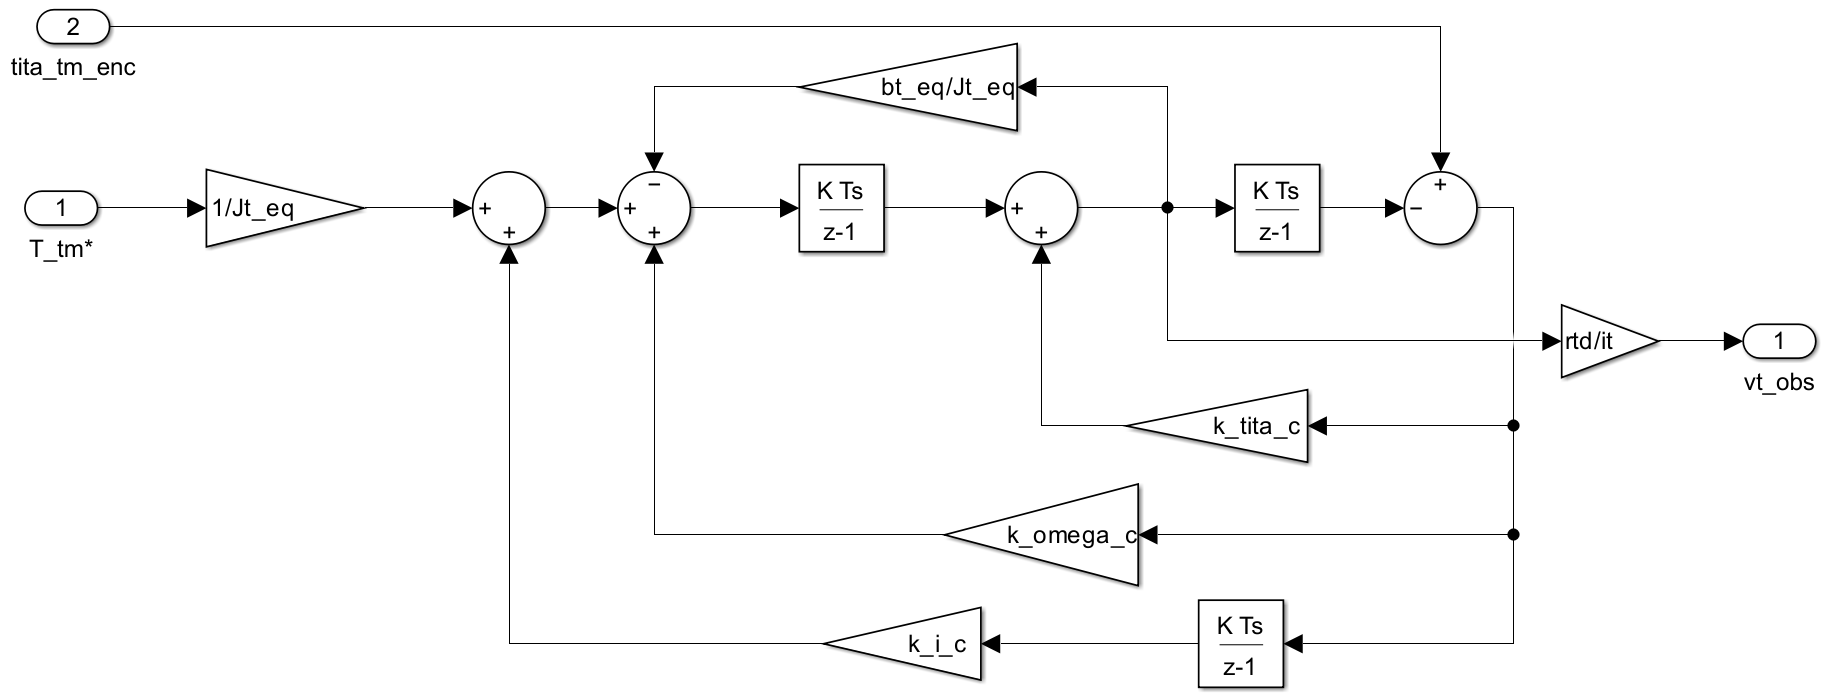
\includegraphics[width=0.9\textwidth]{nivel_2/obs_pid_carro.png}
  
  \vspace{0.2cm}
  \begin{block}{Flujo de señales}
    \begin{itemize}
      \item Encoder → Observador (estima $\tilde{\omega}_{tm}$)
      \item $v_t^*$, $\tilde{\omega}_{tm}$ → PI (calcula $T_{tm}^*$)
      \item $T_{tm}^*$ → Modulador de torque → Planta
    \end{itemize}
  \end{block}
\end{frame}
